%!TEX root = tfintro.tex

\begin{frame}
    \frametitle{Computations as Graphs}
    \framesubtitle{Arithmetic Expressions as a Computation Graph}

    \begin{block}{A Linear Model}
    \begin{columns}
        \begin{column}{0.6 \linewidth}        
            Multiply with weights and add a bias:
            \begin{align*}
                y = W \cdot x + b
            \end{align*}
            Rewritten in function notation:
            \begin{align*}
                y &= +(W \cdot x, b) \\
                  &= +\left(\cdot(W, x), b\right)
            \end{align*}
        \end{column}
        \begin{column}{0.4 \linewidth}
        \begin{figure}[h]
            \centering
            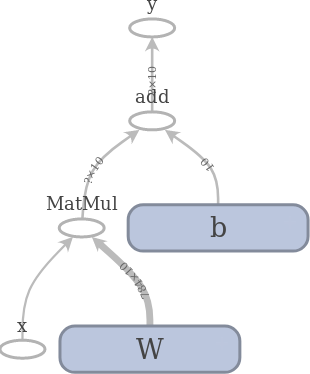
\includegraphics[width=0.45\linewidth]{utils/demo_graph.png}
            \caption{The linear model in graph form.}
        \end{figure}
        \end{column}
    \end{columns}
    \end{block}
    \begin{block}{Operations and Data}
        The expression consists of \operation{operations} that
        are applied to \data{data}:
        \begin{align*}
            y &= \operation{+}\left( \operation{\cdot}(\data{W}, \data{x}), \data{b} \right)
        \end{align*}
        An \operation{operation} is not necessarily a function!
    \end{block}
\end{frame}
    
\begin{frame}
    \frametitle{Why bother?}
    \framesubtitle{Autodifferentiation}
    We don't want to calculate gradients by hand! Use the graph and apply the chain rule automatically.
    %\includegraphics[width=\linewidth]{autodiff}
\end{frame}

\begin{frame}
    \frametitle{Why bother?}
    \framesubtitle{Parallelism}
    \begin{block}{An Ideal World}
    \begin{columns}
    \begin{column}{0.75\linewidth}
        The \data{result} of each \operation{operation} depend only on its input \data{data}. 
        
        Traverse the graph backwards and find all operations whose inputs are \data{data} that is ready.
        These (\operation{a, b, c, d}) can be evaluated in parallel. Whenever an \operation{operation}
        finishes, look if we can start the next one.

        \begin{align*}
            \only<1>{&\operation{f}(\operation{g}(\data{a}, \data{b}), \operation{h}(\data{c}, \operation{d}())}
            \only<2>{&\operation{f}(\data{g}, \operation{h}(\data{c}, \data{d})}
            \only<3>{&\operation{f}(\data{g}, \data{h})}
            \only<4->{&\data{f}}
        \end{align*}
    \end{column}

    \begin{column}{0.25\linewidth}
        \vspace{-2ex}
        \begin{figure}[h]
            \centering
            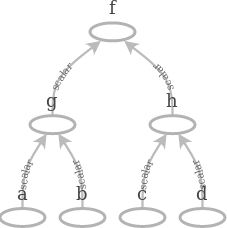
\includegraphics[width=\linewidth]{utils/parallel_graph.png}
            \caption{A parallelizable computation.}
        \end{figure}
    \end{column}
    \end{columns}
    \end{block}

    \begin{block}{The Harsh Reality}<5>
    We want \operation{operations} to be more general than pure functions. Therefore, if one operation depends
    on a side effect of another (but not on data produced by it), we need to add a "fake" (dataless) 
    edge to the graph, called a \emph{\data{control dependency}}.
    \end{block}
\end{frame}

\begin{frame}
    \frametitle{Why bother?}
    \framesubtitle{Efficiency}
    \begin{block}{Acyclic Graphs}
    Calculate only what is needed. Up to now we have considered only trees, but we can use any directed acyclic graph.
    \begin{align}
        x = \operation{f}(\operation{g}(), \operation{h}()), \quad
        y = \operation{s}({\operation{x}(), \operation{h}()}), \quad
        z = \operation{f}(\operation{t}())
    \end{align}
    \end{block}
    \pause
    \begin{block}{Calculation}  
    To calculate $y$ just do the same as before. We will automatically skip useless \operation{operations}
    and compute things only once:
    \only<+>{
    \begin{align}
        x = \operation{f}(\data{g}, \data{h}),\quad
        y = \operation{s}(\operation{x}, \data{h}), \quad
        z = \operation{f}(\operation{t}())
    \end{align}
    }
    \only<+>{
    \begin{align}
        x = \data{f},\quad
        y = \operation{s}(\data{x}, \data{h}), \quad
        z = \operation{f}(\operation{t}())
    \end{align}
    }
    \only<+>{
    \begin{align}
        x = \data{f},\quad
        y = \data{s}, \quad
        z = \operation{f}(\operation{t}())
    \end{align}
    }
    \end{block}
\end{frame}

\begin{frame}
    \frametitle{Why bother?}
    \large{TensorFlow is based on the idea of using a computation graph!}
\end{frame}
